\section{Gray Code}
\label{sec:b-gray}
\source{CSES 2205 (Notion: Bitwise)}{Easy--Medium}

\problemstatement{List all $2^n$ bit strings of length $n\le16$ so that
consecutive strings differ in exactly one bit.}

\begin{patternbox}
Reflected Gray code: $g(i)=i\oplus(i\gg1)$.
\end{patternbox}

\subsection*{Approach and intuition}

Going from $i$ to $i+1$ flips a block of trailing bits: $i=\dots0\,1\,1\cdots1$
becomes $\dots1\,0\,0\cdots0$ (the lowest $0$ and all ones below it). In
$g(i)=i\oplus(i\gg1)$ every bit is the xor of two neighbouring bits of $i$; all
pairs inside the flipped block change on both sides and stay equal, so only the
pair at the top of the block changes. Hence $g(i)$ and $g(i+1)$ differ in
exactly one bit. The map is a bijection (it can be inverted by prefix xor), so
all $2^n$ strings appear.

\begin{center}
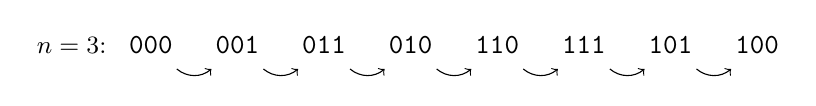
\begin{tikzpicture}[x=1.1cm,y=0.5cm]
\foreach \i/\g in {0/000,1/001,2/011,3/010,4/110,5/111,6/101,7/100}
  \node at (\i,0) {\texttt{\g}};
\foreach \i in {0,...,6} \draw[->] (\i+0.3,-0.6) to[bend right=40] (\i+0.7,-0.6);
\node[left] at (-0.4,0) {\small $n=3$:};
\end{tikzpicture}
\end{center}

\subsection*{Algorithm}
\begin{algorithmic}[1]
\For{$i=0$ \textbf{to} $2^n-1$} print $i\oplus(i\gg1)$ as $n$ bits \EndFor
\end{algorithmic}

\dryrun{$n=2$: $0,1,3,2\to$ \texttt{00, 01, 11, 10}. \checkmark}

\subsection*{C++17 implementation}
\cppfile{bitwise/03_gray_code.cpp}

\begin{complexitybox}
\textbf{Time:} $O(n\,2^n)$ (output size). \textbf{Space:} $O(n\,2^n)$ for
the buffered output.
\end{complexitybox}

\begin{pitfallbox}
\begin{itemize}
  \item Print with leading zeros, most significant bit first.
  \item $2^{16}$ lines $\times$ 17 characters: build one string and print
        once instead of using \texttt{endl} per line.
\end{itemize}
\end{pitfallbox}
